\section{Encoder Pretraining} \label{secs:appendix_encoder_pretraining}
\begin{table*}[t]
\begin{center}
\resizebox{\textwidth}{!}{
\begin{tabular}{@{}lcccccc@{}}
\toprule
\textbf{Model} & \textbf{CoLa}$ (\uparrow$) & \textbf{SST2} ($\uparrow$) & \textbf{RTE} ($\uparrow$) & \textbf{MRPC} ($\uparrow$) & \textbf{QQP} ($\uparrow$) & \textbf{QNLI} ($\uparrow$) \\
\midrule
BERT & 54.6 & 92.5 & 62.5 & 87.6 & 87.4 & 91.0 \\
\midrule
UNITER & 37.4 & 89.7 & 55.6 & 80.3 & 85.7 & 86.0 \\
SimVLM & 46.7 & 90.9 & 63.9 & 84.4 & 87.2 & 88.6 \\
CLIP & 25.4 & 88.2 & 55.2 & 65.0 & 53.9 & 50.5 \\
FLAVA & 50.7 & 90.9 & 57.8 & 86.9 & 87.2 & 87.3 \\
\midrule
Encoder after encoder pretraining & 55.2 & 95.9 & 59.0 & 90.9 & 88.5 & 90.1 \\
\midrule
Encoder after encoder-decoder training \\
\quad (w/o encoder pretraining) & 15.7 & 82.5 & 49.5 & 81.5 & 76.8 & 66.6  \\
\quad (w/ encoder pretraining) & 20.4 & 84.8 & 53.4 & 78.3 & 76.7 & 78.2  \\
\bottomrule
\end{tabular}
}
\caption{Results of \bdraw text encoder on the GLUE benchmark after pretraining with joint BERT and CLIP objectives or (continued) training with text-to-image generation objective.}
\label{table:glue_results}
\end{center}
\end{table*}

\begin{figure}[ht!]
    \centering        
    \setlength{\tabcolsep}{2.0pt}      
    \begin{tabular}{ccccc} 
        \rotatebox{90}{\scriptsize\phantom{AA} No Encoder Pretrain} &                    
        
\includegraphics[width=0.19\textwidth]{figures/enc_pretrain/enc_pretrain_0_0.jpg} &
        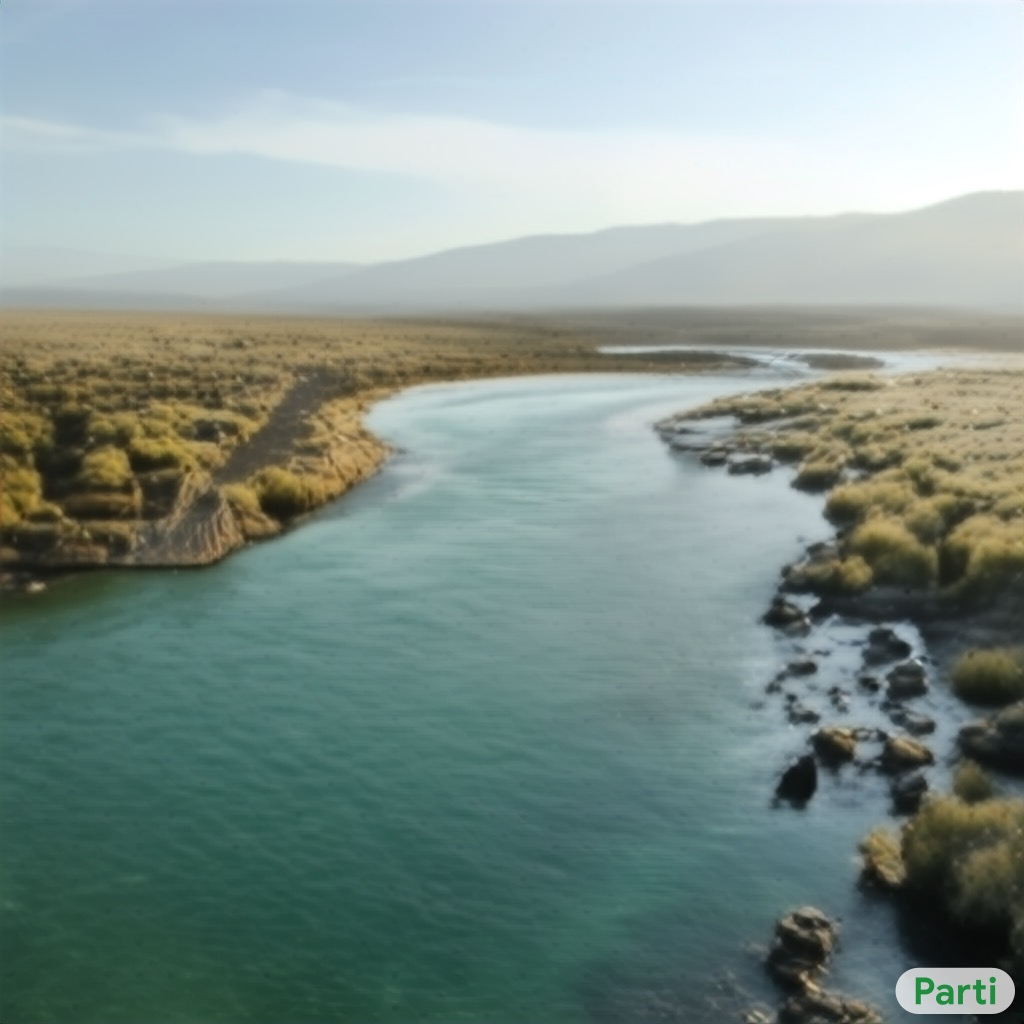
\includegraphics[width=0.19\textwidth]{figures/enc_pretrain/enc_pretrain_1_0.jpg} &
        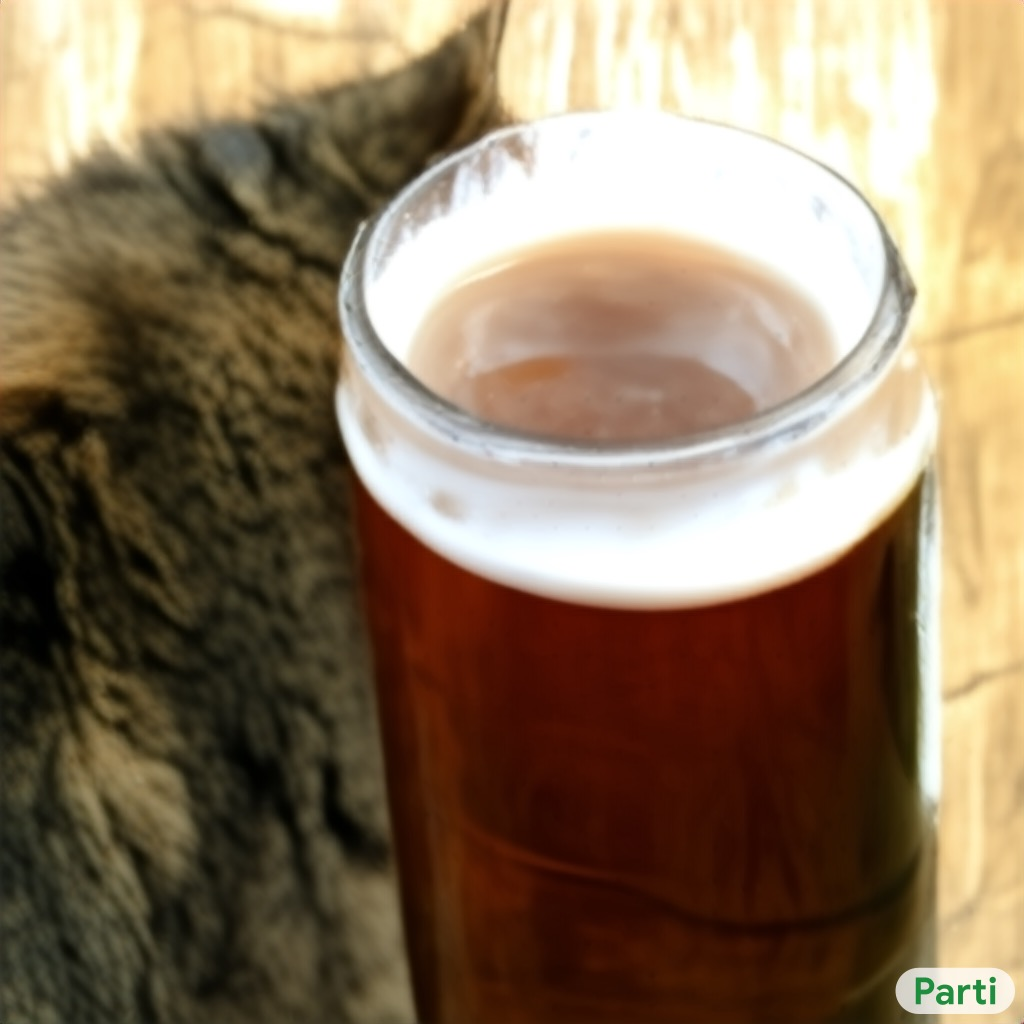
\includegraphics[width=0.19\textwidth]{figures/enc_pretrain/enc_pretrain_2_0.jpg} &
        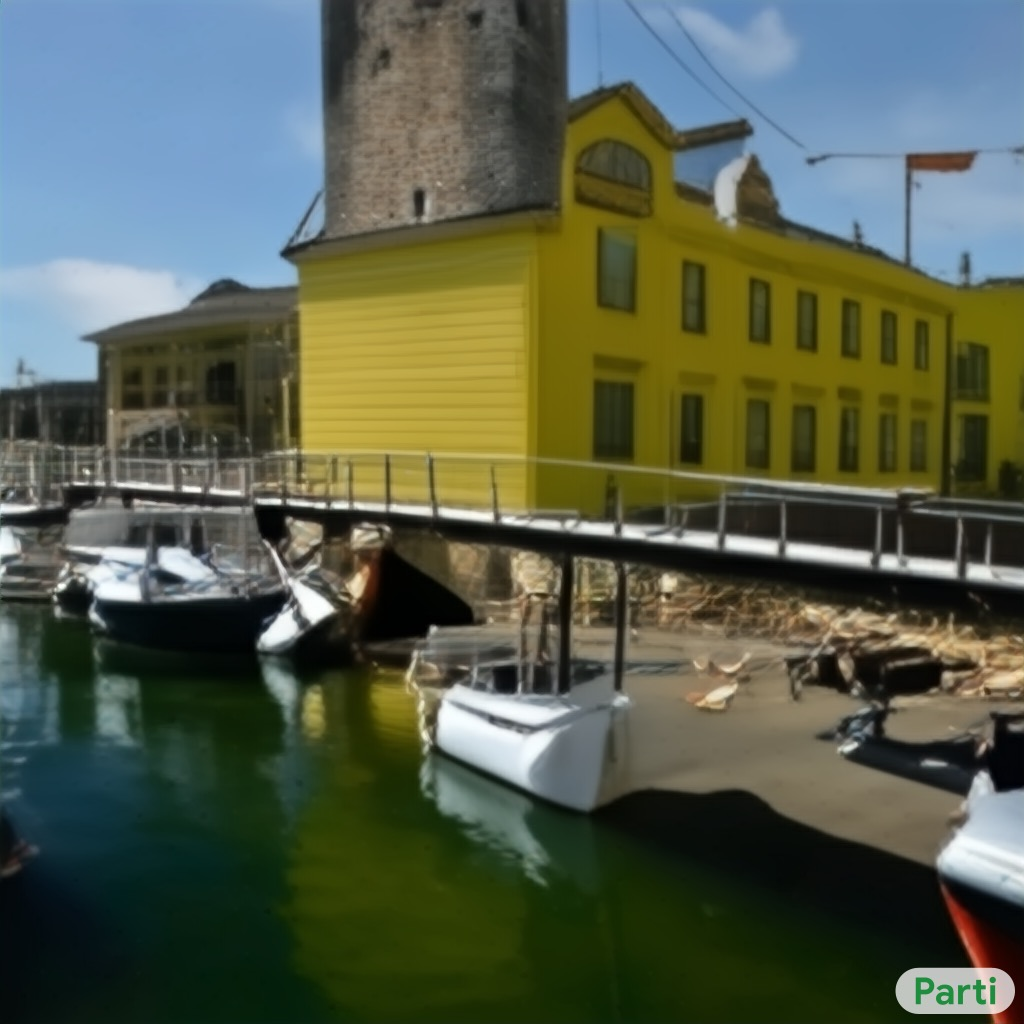
\includegraphics[width=0.19\textwidth]{figures/enc_pretrain/enc_pretrain_6_0.jpg} \\
                                                                                    
        \rotatebox{90}{\scriptsize\phantom{AA} Encoder Pretrain} &            
        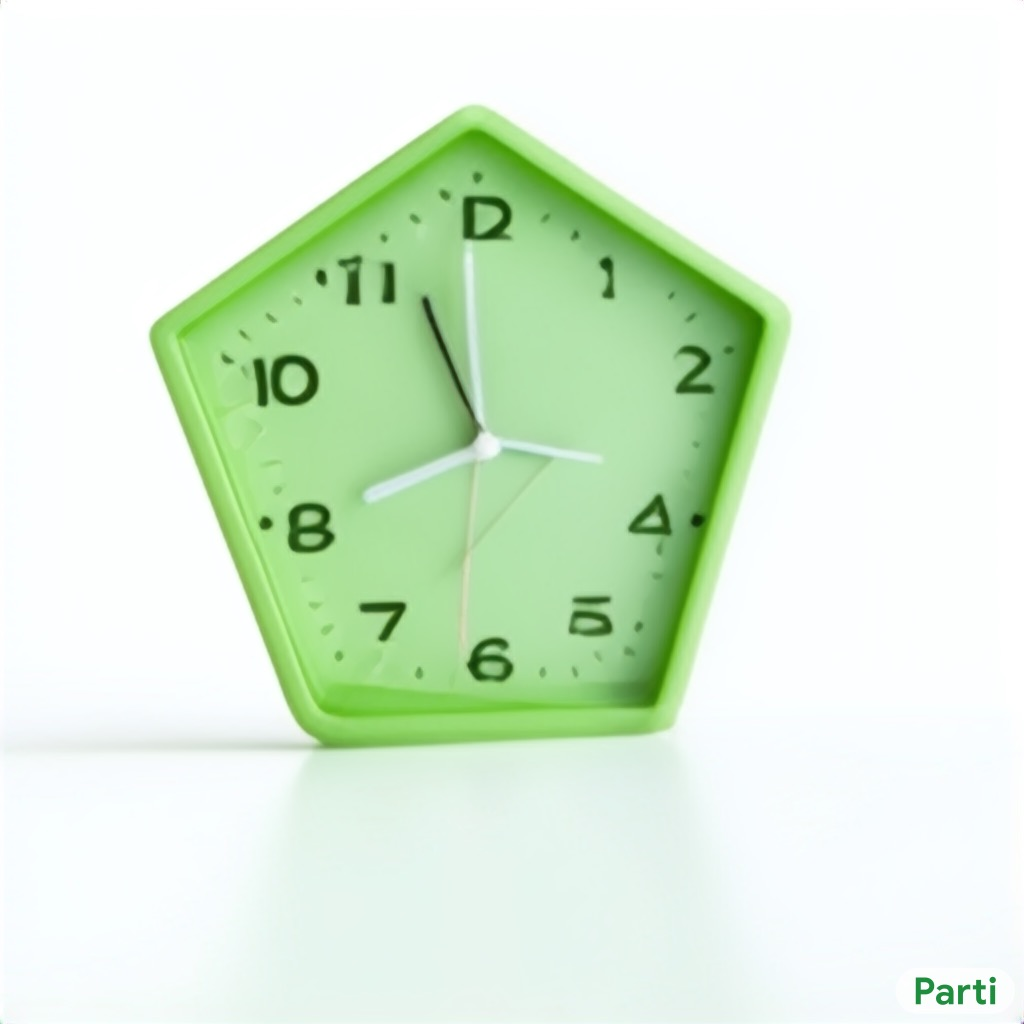
\includegraphics[width=0.19\textwidth]{figures/enc_pretrain/enc_pretrain_0_1.jpg} &
        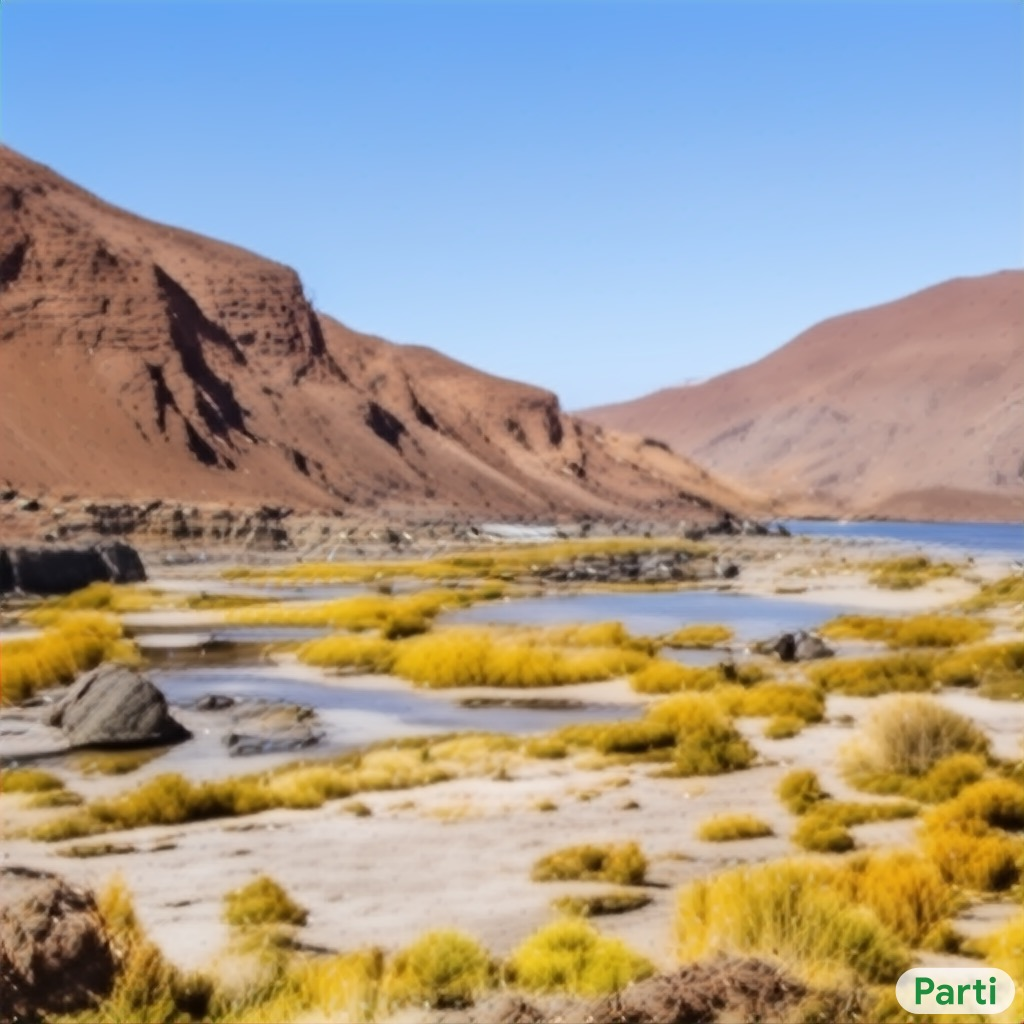
\includegraphics[width=0.19\textwidth]{figures/enc_pretrain/enc_pretrain_1_1.jpg} &
        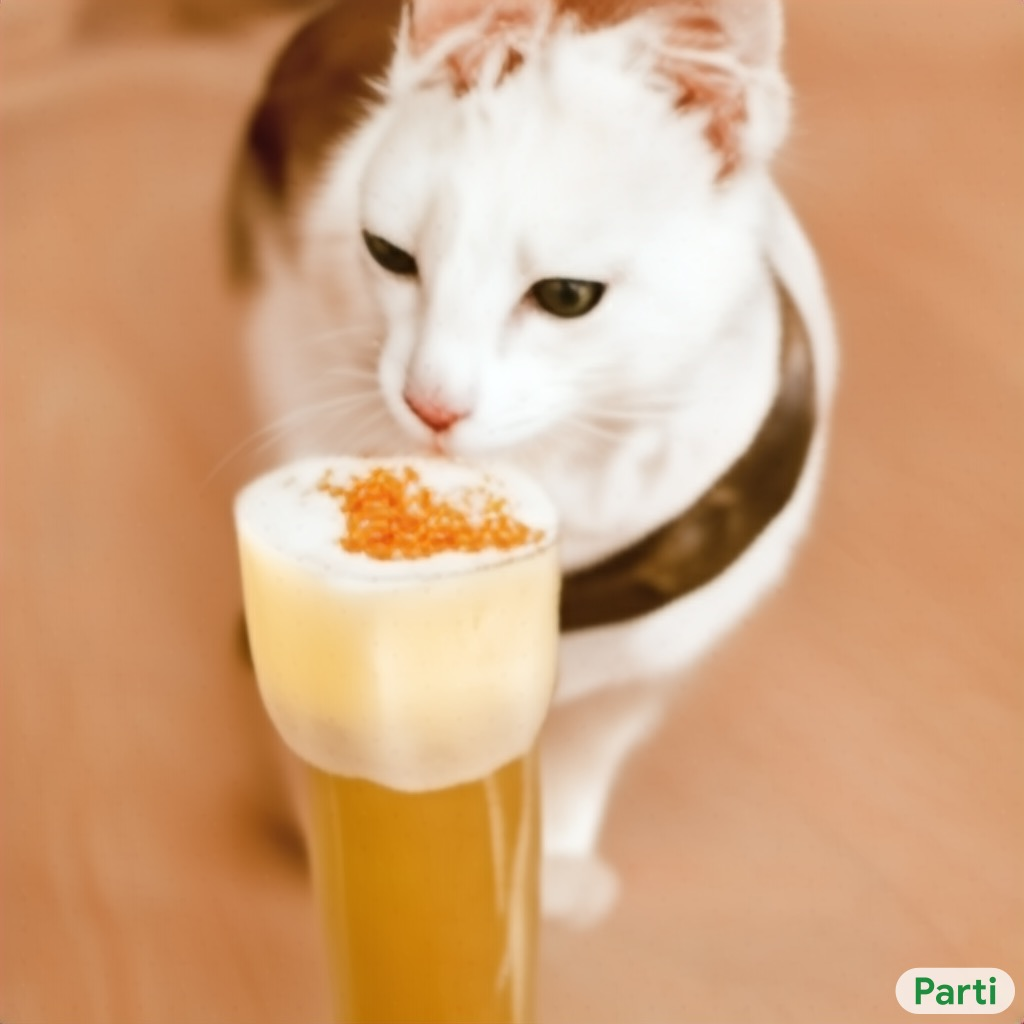
\includegraphics[width=0.19\textwidth]{figures/enc_pretrain/enc_pretrain_2_1.jpg} &
        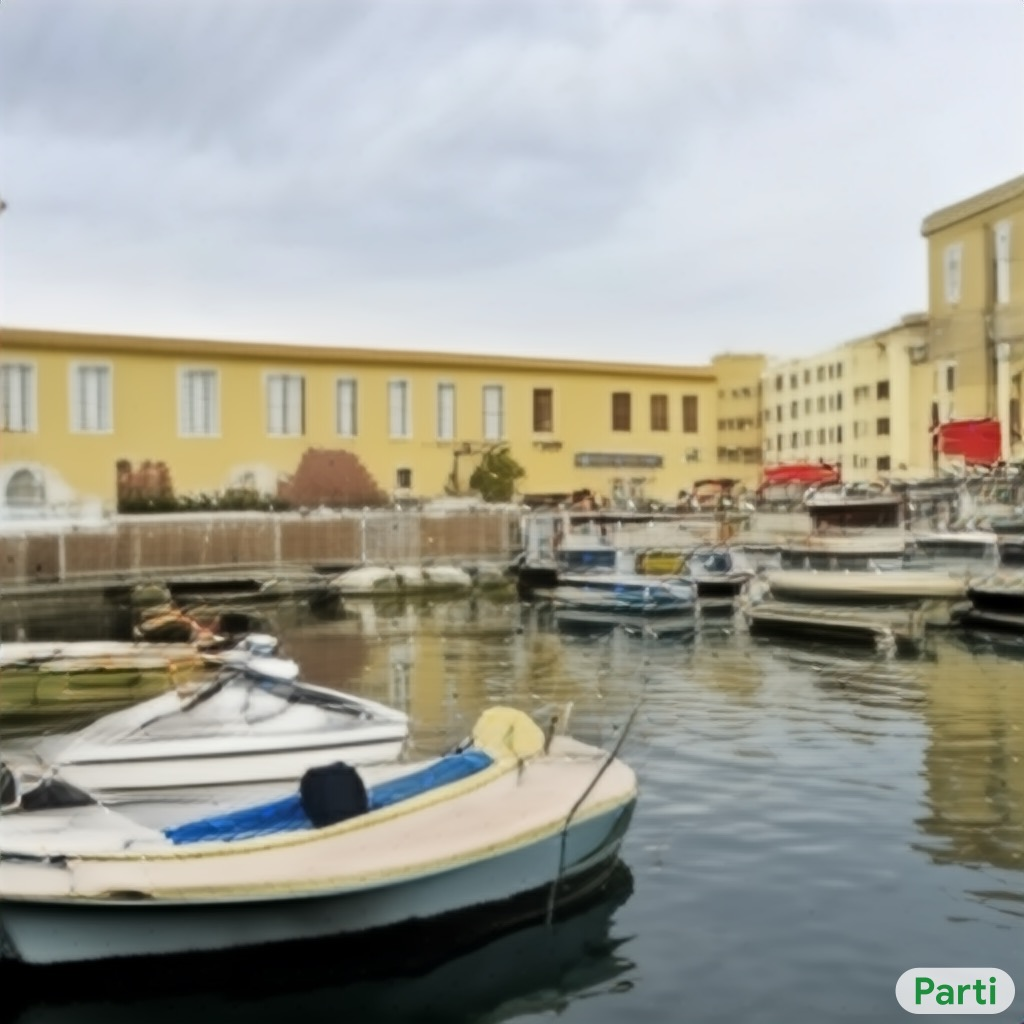
\includegraphics[width=0.19\textwidth]{figures/enc_pretrain/enc_pretrain_6_1.jpg} \\

        & \scriptsize \makecell{``a green clock in \\ the shape of a pentagon.''} 
        & \scriptsize \makecell{``a winding river \\ crosses the atacama desert.''}
        & \scriptsize \makecell{``a cat drinking \\ a pint of beer.''}          
        & \scriptsize \makecell{``a group of boats in \\ a harbor docked next to \\ a yellow building.''} \\
    \end{tabular}                                                                   
    \caption{Ablation of text encoder pretraining. In some of the prompts, we observe text-pretrained model outperforms non-pretrained encoders as examples shown above. However on average, we observe \textit{no significant} quality improvement by warming-up text encoder. Both models are with 3B parameters trained on the same mixture of datasets for ablation.}
    \label{figs:enc_pretrain}
\end{figure}

\begin{figure}[!ht]
\centering
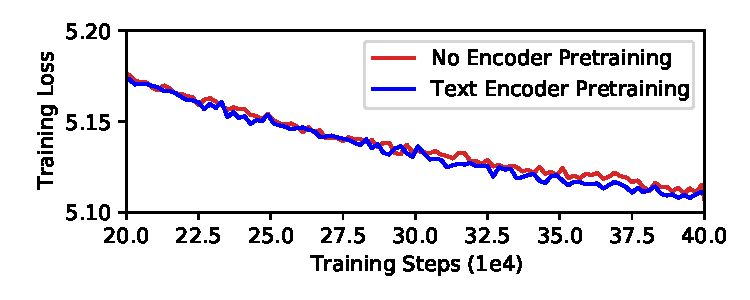
\includegraphics[width=0.8\textwidth]{figures/text_pretraining_losscurve.pdf}
\caption{Ablation of text encoder pretraining. We plot text-to-image generation softmax cross-entropy training loss. The training of pretrained text encoder is only slightly better. Both models are with 3B parameters trained on the same mixture of datasets for ablation.}
\label{figs:text_pretrain_loss}
\end{figure}

While it is straightforward to warm-start the model with a pretrained text encoder, we observe the text-encoder pretraining \textit{very marginally} helps text-to-image generation loss with 3B-parameter \bdraw models. Qualitative examples are shown in Figure~\ref{figs:enc_pretrain} and quantitative loss comparison is shown in Figure~\ref{figs:text_pretrain_loss}. We leave this observation as a future research topic on the difference and unification of generic language understanding and visually-grounded language understanding.